%----------------------------------------------------------------------------------------
%	LAB BOOK CONTENTS
%----------------------------------------------------------------------------------------

\labday{Friday, 1 April, 2016}
\begin{enumerate}
  \item Tried to find reasonable value for the heating rate in the energy equation for the zero-D reactor.
  \item Finally got Drekar configured and compiled.  All tests, including extended tests, pass.  Errors when adding options for SUPG Energy evaluator.  Not clear what the errors are.
\end{enumerate}

%-----------------------------------------
\experiment{0D Reactor}
To do:
\begin{enumerate}
  \item Clean up code.  Add comments and document how it works.
  \item Find reasonable heating rate values.
  \item Run heating rate calibration.
\end{enumerate}
Today I just worked on the heating rate values.
%-----------------------------------------
\subexperiment{Heating Rate}
Recall that the energy equation is
\begin{align}
  \odeone{T}{t} = -\dfrac{\displaystyle\sum_{k=1}^{N}{u_{k}\lr{T}\odeone{x_{k}}{t}}}{\displaystyle\sum_{i=k}^{N}{c_{vk}x_{k}}} + Q_{T}
\end{align}
where $T$ is the temperature, $u_{k}\lr{T}$ is the internal energy of species $k$, $x_{k}$ is the molar concentration of species $k$ and $c_{vk}$ is the specific heat at constant volume of species $k$.  We have also included the heating rate $Q_{T}$ which may be a function of time or temperature.

\begin{tcolorbox}[colback=blue!5, colframe=blue!40!black, title=Estimate of Heating Rate]
  \begin{align*}
    Q_{T} \approx \odeone{T}{x}s_{L}
  \end{align*}
  where $s_{L}$ is the laminar flame speed.
\end{tcolorbox}

The laminar flame speed for hydrogen-air premixed flames at $\phi = 1$ is approximately $2$ m/s.  The energy equation in one dimension reduces to
\begin{align}
  \rho s_{L}\odeone{T}{x} = \odeone{}{x}\lr{\frac{\lambda}{c_{p}} \odeone{T}{x}}
\end{align}
where we assumed constant specific heat among species and no reactions.  Integrating this from $T_{u}$ to $T_{b}$ and solving for the temperature gradient gives
\begin{align}
  \odeone{T}{x} = \frac{\rho_{u}c_{p}s_{L}}{\lambda_{b}}\lr{T_{b}-T_{u}}.
\end{align}
Hence,
\begin{align}
  Q_{T} \approx \frac{\rho_{u}c_{p}s_{L}^{2}}{\lambda_{b}}\lr{T_{b}-T_{u}}.
\end{align}
If we now use some very rough values for air of $\rho_{u} = 1.225$, $c_{p} \approx 1200$ and $\lambda_{b}=0.05$ and we use $T_{b}\approx 3000$, $T_{u} = 1500$ with $s_{L}=4$ (all in SI units and temperatures in Kelvin) then $Q_{T}\approx 10^{8}$.  Note that $T_{b}$ and $T_{u}$ were taken from a simulation of the 0-D reactor without any source term.

%-----------------------------------------
\experiment{VMS-ThermalConv}
Worked on building Drekar.

\subexperiment{Building Drekar}

\labday{Week of April 4th, 2016}
\begin{itemize}
  \item Spent the week in Lausanne, Switzerland at SIAM UQ 16.  Made some notes about papers to read.  Will hopefully read some of them on the plane ride home.
  \item Thought about what plots to include in Janus particle paper but did not finish this.  Here's what I need to get:
    \begin{enumerate}
      \item Plot of $U\lr{t}$ for advection and no-advection cases with same values of $\alpha$ and $C$.
      \item Plot of logarithmic decay for no-advection case.
      \item Plots illustrating qualitative behavior of solution such as:  $U\lr{t}$ at for constant $C$ and various values of $\alpha$, $U\lr{t}$ for constant $\alpha$ and various values of $C$, illustration of different qualitative regimes such as peak velocity or not, plots of $t_{max}$ with $C$ and $\alpha$ when appropriate, relationship between final swimming velocity and $\alpha$ and $C$.
    \end{enumerate}
  \item Got motivated to use \fenics to do some tests of the old non-diagonal stabilization parameter.  First implement linear Burger's MHD (constant advection velocity and magnetic field coefficient), then do full Burger's MHD.  These tests will be \textit{steady} for now.  Then, when the solution looks decent, put in GLS stabilization and check solution again with the usual diagonal stabilization parameter.  Finally, put in the new non-diagonal stabilization parameter and compare the solutions.  If the solutions look good (which they should since we've done this before) then try out some two dimensional problems.  Will need to code up the full MHD equations.  Try to do Hartmann flow perhaps?  There may be some other interesting ones to try too.
\end{itemize}

\experiment{0D Reactor}
I didn't get to work on this, but here is a list of things to do:
\begin{enumerate}
  \item Get heating rate calculations going.  Just need to get that version of the code cleaned up a bit, but otherwise it should be ready to go.
  \item Clean up general code for distribution.
    \begin{enumerate}
      \item Add better comments and remove junk comments.
      \item Get ready to send forward problem version out without stochastic operator.  Make sure there is no clash between Rebecca's loop over initial temperatures and the heating rate version.  Could probably just give a flag here.  If someone specifies both a heating rate and various initial temperatures then throw an error.
      \item Prep the stochastic operator version without calibration.  We will provide the calibrated parameters and they can just run the code with those parameters.
      \item Figure out how to give them a version of the code that they can calibrate \textit{without} \texttt{QUESO}.
    \end{enumerate}
    \item Set up $\ce{NO_x}$ reactions:
      \begin{align*}
        \ce{N2 + O <--> NO + N} \\
        \ce{N + O2 <--> NO + O} \\
        \ce{N + OH <--> NO + H}
      \end{align*}
      The ODEs for these reactions will use \ce{N2}, \ce{O}, \ce{OH}, and \ce{H} as data and will be solved for \ce{NO} and \ce{N}.
    \item Change from constant volume energy equation to constant pressure energy equation.  It could be as simple as
      \begin{align*}
        H = \sum_{i=1}^{n_{react}}{h_{i}\lr{T}x_{i}}
      \end{align*}
      and $\dfrac{\mathrm{d}H}{\mathrm{d}t} = 0$.  Then we'll just have enthalpies insteady of internal energies and $c_{p}$ instead of $c_{v}$.
\end{enumerate}

%-----------------------------------------
\labday{April 9th, 2016}
Flying back from Switzerland now.  Somewhere over the Atlantic (probably middle).  Working on compiling Janus particle results.

\experiment{Janus Particles}
Basically just did a parameter sweep over $\alpha$ and $C$ to determine how the final swimming velocity is affected by the parameters.  Save the data in \texttt{ascii} format as text files and made plots in Python.  Need to clean this up.  One thing I noticed is that the swimming velocity maybe have multiple maxima when it overshoots.  This probably precludes the original goal of plotting the time to maximum as a function of the parameters.  Still want to plot logarithmic decay of the case with no advection but this didn't go quite right.  Either way, I now have the data to compare swimming velocity with and without advection.  Another interesting thing to do may be to add in a non-symmetric coating function.  It'd be nice to have a ramp up and then quick decay.  Some combination of exponentials should do the trick.

\labday{Wednesday, 27 April, 2016}
Got a bit behind on the notebook.  Here are some of the main things that I've been working on.  First of all, the 0D reactor has been uploaded to the Bitbucket repo.  Here are the problemls that have been uploaded:
\begin{enumerate}
  \item Forward problem including both the reduced and detaile models.
  \item Calibration of the reduced model.  Our version using \texttt{Queso} as well as a stripped down version have been provided.  The stripped down version requires the user to provide their own software for the inverse problem and QoI.
  \item The inadequacy operator.  Our version using \texttt{Queso} as well as a stripped down version have been provided.  Once again, the stripped down version requires the user to provide their own software for the inverse problem and the QoI.
\end{enumerate}
Documentation for all of these problems has been provided.  Each file has been extensively commented, cleaned up and in some cases refactored.  New input files have also been created to help mitigate the amount that the user much recompile.

I've been working on the calibration design for the heating rate problem.  I wrote a script that samples the parameter set $\left\{A, b, E_{a}\right\}$ and computes the ignition temperature for each set.  The resulting distribution is shown in figure~\ref{fig:Tig}.
\begin{figure}[h]
  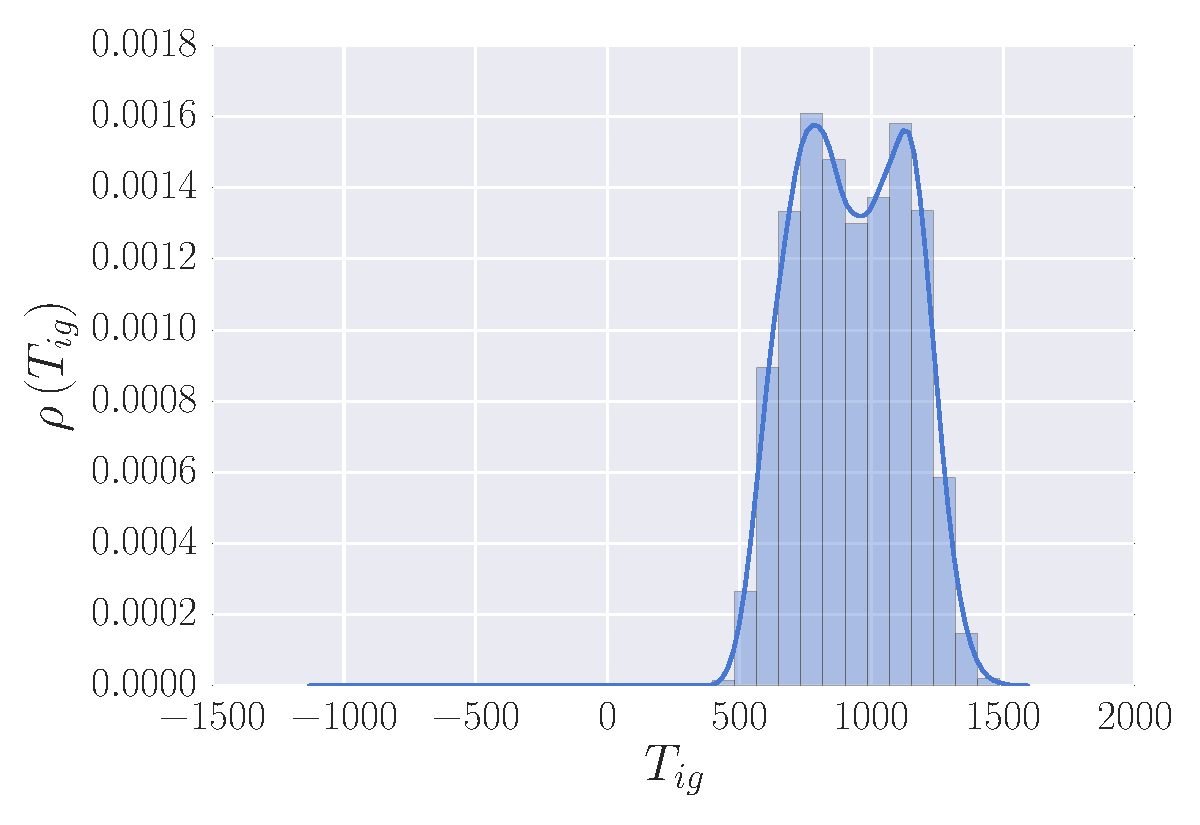
\includegraphics[width=\textwidth]{figures/2016/April/Ignition_Temperature.pdf}
  \caption{Distribution of ignition temperatures.  The negative values are due to not integrating for long enough or not starting at a low enough temperature.}
  \label{fig:Tig}
\end{figure}
The next step is to actually perform the calibration.  First, run the detailed model to get a feel for how many sample points to run.  Based on the ignition temperature distribution, it probably makes sense to start at $T_{0}\approx 450$.  However, we don't want too many points sampled before ignition.  Hence, some trial and error may be necessary here.  We also need to make sure that we sample enough in the sharp layer after ignition.  The current $\Delta t$ should be sufficient for this ($\Delta t = 5\times 10^{-6}$).  May also be useful to run at one or two different heating rates to make sure the heating rate does not affect things too much.  The calibration will then just be run over a range of equivalence ratios ($\phi$).

A few notes on distributions.  The normal distribution with mean $\mu$ and standard deviation $\sigma$ is
\begin{align*}
  \mathcal{N}\lr{x; \mu, \sigma^{2}} = \frac{1}{\sigma\sqrt{2\pi}}\exp\lr{\frac{\lr{x-\mu}^{2}}{2\sigma^{2}}}.
\end{align*}
We can compute the expected value as follows.
\begin{align*}
  \mathbb{E}\lr{x} &= \int_{-\infty}^{\infty}{x\mathcal{N}\lr{x;\mu, \sigma} \ \mathrm{d}x} \\
                   &= \frac{1}{\sigma\sqrt{2\pi}}\int_{\infty}^{\infty}{x\exp\lr{\frac{\lr{x-\mu}^{2}}{2\sigma^{2}}} \ \mathrm{d}x} \\
                   &= \frac{1}{\sigma\sqrt{2\pi}}\int_{\infty}^{\infty}{\lr{u+\mu}\exp\lr{-\frac{u^{2}}{2\sigma^{2}}} \ \mathrm{d}u} \\
                   &= \frac{1}{\sigma\sqrt{2\pi}}\left[\int_{-\infty}^{\infty}{u \exp\lr{-\frac{u^{2}}{2\sigma^{2}}}\ \mathrm{d}x} + \int_{-\infty}^{\infty}{\mu \exp\lr{-\frac{u^{2}}{2\sigma^{2}}}\ \mathrm{d}x}\right] \\
                   &= \frac{1}{\sigma\sqrt{2\pi}}\left[0 + \mu \sigma\sqrt{2\pi}\right] \\
                   &= \mu.
\end{align*}

Another distribution that we use a lot is the lognormal distribution.  The idea is that the logarithm of the random variable is normally distributed.  We denote this by
\begin{align*}
  \ln\mathcal{N}\lr{x; \mu, \sigma} = \frac{1}{\sigma\sqrt{2\pi}}\int_{0}^{\infty}{\frac{1}{x}\exp\lr{\frac{\lr{\ln\lr{x} - \mu}^{2}}{2\sigma^{2}}} \ \mathrm{d}x}.
\end{align*}
Note that the random variable $x > 0$.  We can compute the mean as follows.
\begin{align*}
  \mathbb{E}\lr{\ln\mathcal{N}\lr{x; \mu, \sigma}} &= \frac{1}{\sigma\sqrt{2\pi}}\int_{0}^{\infty}{\exp\lr{\frac{\lr{\ln\lr{x} - \mu}^{2}}{2\sigma^{2}}}\ \mathrm{d}x} \\
     &= \frac{1}{\sqrt{\pi}}\int_{-\infty}^{\infty}{e^{\mu}\exp\lr{\sqrt{2}\mu u}\exp\lr{-u^{2}} \ \mathrm{d}u}
\end{align*}
where we have used the substitution
\begin{align*}
  u = \frac{\ln\lr{x} - \mu}{\sqrt{2}\sigma}.
\end{align*}
Completing the square
\begin{align*}
  -u^{2} + \sqrt{2}\sigma u = -\left[\lr{u - \dfrac{\sigma}{\sqrt{2}}} - \dfrac{\sigma^{2}}{2}\right]
\end{align*}
results in
\begin{align*}
  \mathbb{E}\lr{\ln\mathcal{N}\lr{x; \mu, \sigma}} &= \frac{1}{\sqrt{\pi}}\exp\lr{\mu}\exp\lr{\frac{\sigma^{2}}{2}}\int_{-\infty}^{\infty}{\exp\lr{-\lr{u - \frac{\sigma}{\sqrt{2}}}^{2}}\ \mathrm{d}u} \\
  &= \exp\lr{\mu + \frac{\sigma^{2}}{2}}.
\end{align*}
%-----------------------------------------
%\end{addmargin}

\end{document}



























